\section{一维离散映射系统:Logistic映射}
Logistic映射是研究动力系统、混沌、分形等复杂系统的一个经典模型,其来源于生态学中的虫口模型,用以描述种群的变化。Logistic映射从数学形式上来看是一个非常简单的混沌映射,但却有极其复杂的动力学行为,在保密通信领域的应用十分广泛。

Logistic是一个定义在$x\in [0,1]$的一维离散的动力系统,其动力学方程可描述为
\begin{equation}
    x_{n+1}=f(x_n)=\gamma x_n(1-x_n),\ x_n\in [0,1], n=1,2,3,\cdots
\end{equation}
Logistic映射存在两个不动点:$x_1^*=0$和$x_2^*=1-\frac{1}{\gamma}$。Logistic映射的相图描述了相空间的映射关系:
\begin{figure}
	\centering
	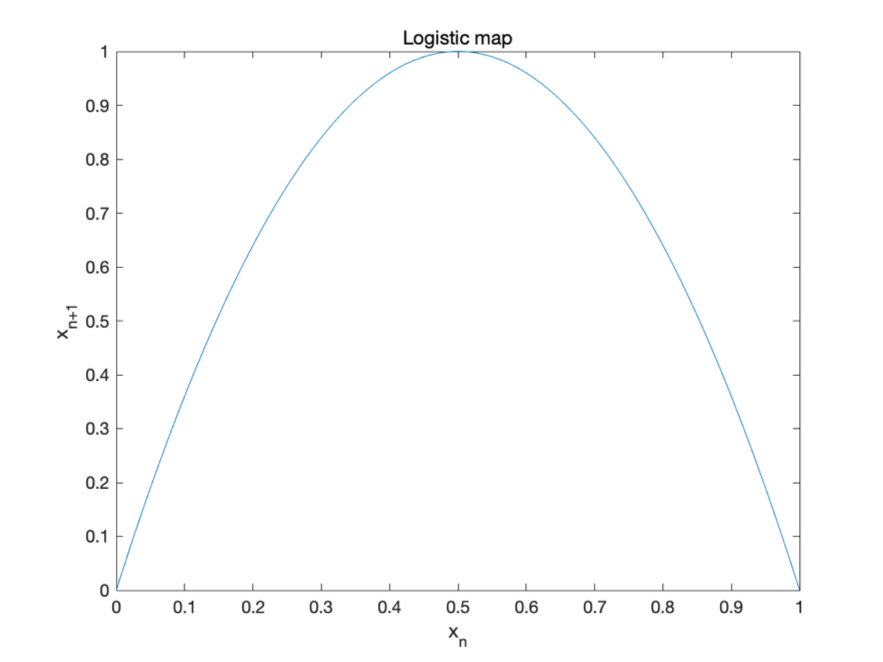
\includegraphics[scale=0.6]{logistic_phase.png}
    \caption{Logistic映射的相图($\gamma=4$)}
    \label{fig:logi_pha}
\end{figure}

Logistic映射的动力学过程可以看作是在一维相空间上的拉伸再折叠的过程。通过非线性动力学的知识可以得到,该系统在$\gamma$取不同值时表现出不同的动力学行为。当$0<\gamma<1$时,系统最终都会渐进的趋于0;当$1<\gamma<3$时,系统会收敛到一个不动点,该不动点的值为$x^*=(\gamma-1)/\gamma$,此时系统的极限行为会趋于该不动点的值;当$3<\gamma<3.57$时,系统的迭代会出现周期行为,随着$\gamma$的增大,周期的长度也会相应的增加,例如2周期,4周期,8周期轨道等,直到大约为$\gamma=3.57$时,周期的长度趋于无穷大;当$3.57<\gamma<4$时,系统的迭代会在周期类型和混沌类型之间来回切换,且大部分区域呈现混沌状态;直到$\gamma=4$时,系统处于完全混沌的状态。

Logistic映射的分岔图$x_n-\gamma$描述了系统随$\gamma$表现出的不同的动力学行为:
\begin{figure}
	\centering
	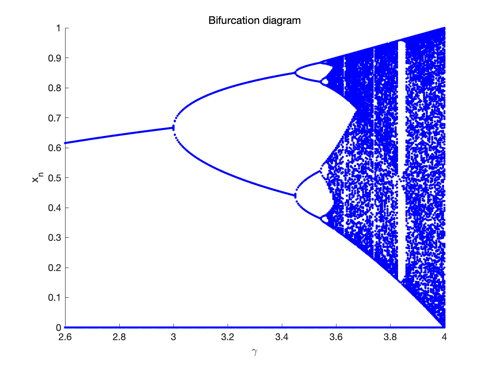
\includegraphics[scale=1]{logistic_bifurcation.png}
    \caption{Logistic映射的分岔图($2.6\leqslant\gamma\leqslant 4$)}
    \label{fig:logi_pha}
\end{figure}

李雅普诺夫指数是描述混沌现象的一个重要的指标,Logistic映射的李雅普诺夫指数图像$\lambda-\alpha$如下图所示:
\begin{figure}
	\centering
	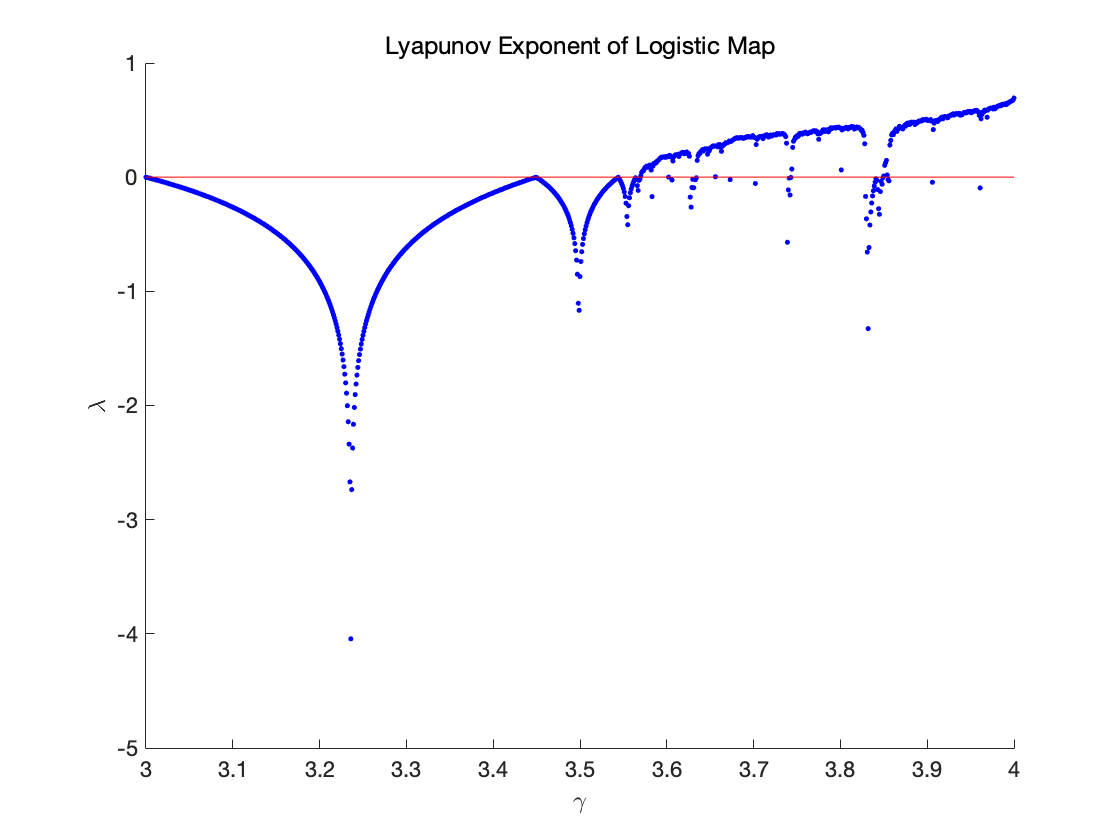
\includegraphics[scale=0.2]{logistic_lypn.png}
    \caption{Logistic映射的李雅普诺夫指数}
    \label{fig:logi_lypn}
\end{figure}
根据李雅普诺夫指数的性质:当$\lambda<0$时,映射系统收敛于某一不动点;当$\lambda=0$时,系统进行周期运动;当$\lambda>0$时,系统处于混沌状态。我们可以同样得到在$3.57<\gamma<4$区域,系统处于混沌状态(在$\gamma=3.83$处存在一三周期轨道),当$\gamma=4$时系统处于混沌状态。

不失一般性,在我们的Koopman分析中,我们取$\gamma=4$的一个特例,通过Logistic映射的动力学方程演化出一系列的数据,作为Koopman分析的源数据,以此来分析Logistic映射的系统特征。